\documentclass[a4paper, 13pt]{article}
\usepackage[left=2cm,right=2cm,top=2cm,bottom=2cm]{geometry}
\setlength{\parindent}{1.5cm}
\usepackage{graphicx}
\usepackage{kvsetkeys}
\begin{document}

\title{MM2090 Assignment-4}
\author{Abhaumika Bijudith ME20B004}
\date{July 2021}
\maketitle

\section{The Equation}




Hall Effect  :  

\begin{equation}
 {\LARGE{\textbf{$V =\frac{Bi}{{ned}}$}}}
 \label{eqn:equation}
\end{equation}


\subsection{Analysis}
Following contains a brief explanation of the variables and the importance of the equation :
\begin{itemize}

    {\normalsize {The above given equation \ref{eq:1}  has terms \textbf{V} ,\textbf{B} , \textbf{i} ,\textbf{n} ,\textbf{e} and  \textbf{d}.}}

{\normalsize { Here,}}\\
{\normalsize {\textbf{V} represents the voltage across the two plates }}\\
{\normalsize {\textbf{B} \  represents the magnetic field between the two plates}}\\
{\normalsize {\textbf{i} \  represents the current flowing between the two plates}}\\
{\normalsize {\textbf{n} \  represents the density of charge carrier}}\\
{\normalsize{\textbf{e} \ represents the electronic charge}}\\
{\normalsize{\textbf{d} \ represents the distance between the two plates}}
\end{itemize}


The Hall effect is the production of a voltage difference (the Hall voltage) across an electrical conductor that is transverse to an electric current in the conductor and to an applied magnetic field perpendicular to the current. It was discovered by Edwin Hall in 1879.

A Hall effect can also occur across a void or hole in a semiconductor or metal plate, when current is injected via contacts that lie on the boundary or edge of the void or hole, and the charge flows outside the void or hole, in the metal or semiconductor. This Hall effect becomes observable in a perpendicular applied magnetic field across voltage contacts that lie on the boundary of the void on either side of a line connecting the current contacts, it exhibits apparent sign reversal in comparison to the standard ordinary Hall effect in the simply connected specimen, and this Hall effect depends only on the current injected from within the void.

\begin{figure}[h]
	{\begin{center}
		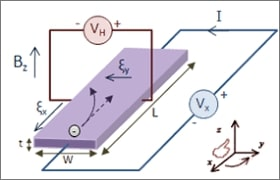
\includegraphics[scale=0.45]{ME20B004.jpg}
	\end{center}}
	\caption{Hall Effect \cite{pic}}
	\label{f1:image}
\end{figure}

Webpage Links \cite{weblink}



%\bibliography{bibliography.bib}
%\bibliographystyle{plain}

\end{document}
